\documentclass{acm_proc_article-sp}

%packages
\usepackage{epstopdf}
\usepackage{hyperref}
\usepackage{tikz}
\usepackage{algpseudocode}
\usepackage{algorithm}
\usepackage{cleveref}
\usepackage{todonotes}
\usepackage{cite}
\usepackage{pgfplots}
\usepackage{microtype}
\usepackage{siunitx}
\usepackage{tikz}
\usetikzlibrary{arrows,automata}
\usepackage{siunitx}
\usepackage{pgf}
\usepackage{titlesec}

%set spacing before and after \sections and \subsections
\titlespacing*{\section}
{0pt}{3ex}{3ex}
\titlespacing*{\subsection}
{0pt}{3ex}{3ex}

\usetikzlibrary{arrows}

 
\DeclareSIUnit\Wh{Wh}
\DeclareSIUnit\miles{mi}


\begin{document}

\title{Fastest-Path Algorithm for Electrical Vehicles}

\numberofauthors{4} 
\author{
% 1st. author
		\alignauthor A. B. Eriksen\\
       \affaddr{Institute of Computer Science}\\
       \affaddr{Aalborg University}\\
       \email{aeriks11@student.aau.dk}
% 2nd. author
		\alignauthor M. A. Madsen\\
       \affaddr{Institute of Computer Science}\\
       \affaddr{Aalborg University}\\
       \email{mman10@student.aau.dk}
\and
% 3rd. author
		\alignauthor
		M. M. Andersen\\
       \affaddr{Institute of Computer Science}\\
       \affaddr{Aalborg University}\\
       \email{mama11@student.aau.dk}
% 4th. author
		\alignauthor
		S. B. Jensen\\
       \affaddr{Institute of Computer Science}\\
       \affaddr{Aalborg University}\\
       \email{sbje11@student.aau.dk}}
\date{30 July 2014}
\maketitle

\begin{abstract}
We describe a greedy heuristic algorithm for finding the fastest path, between two points in a
large road network graph, for electric vehicles (EVs). We further introduce a linear programming 
approach, which could be combined with the greedy heuristic algorithm and likely improve fastest path 
finding abilities at the cost of run time performance. Unlike many of today's GPS systems, the greedy heuristic 
algorithm takes both the drive time and the recharge time into account. Since the recharging possibilities for 
electric vehicles are still limited on Danish roads and the recharging process takes a long time compared to refuelling 
times of regular gasoline cars, this is necessary in order to give the electric vehicles users a 
useful route plan.\\

We compared the performance of the greedy heuristic algorithm with a naive algorithm on road
networks extracted from OpenStreetMap (OSM). We modified the OSM road network, so it contained Danish speed limits
and charge stations at variable positions and with variable charge rates. We compared the performance of the algorithms 
with four different parameters: the density of charge stations in the road network, the charge rates of the charge stations 
in the road network, the size of the road network measured in distance and the complexity of the road network measured 
in number of nodes. HOW DID IT PERFORM?!      

\end{abstract}

\keywords{Shortest-path algorithm with resource constraints, Electrical vehicles, Road-network, Route planing} % NOT required for Proceedings

\section{Introduction}

As the adoption rate of electric vehicles increases \cite{Henry2013}, the need for a better and more complex route planing solution appears. Electric vehicles generally have a shorter range as well as a significantly slower recharge time, compared to traditional gasoline cars. As the recharge time have become a significant factor in the total travel time, the time spend recharging should be taken into account by a route planning system, to accommodate for an otherwise large margin of error. Time spend recharging batteries is inherently variable, as the charge rate is affected by both the charge station's charge rate as well as the battery's current charge. When planning a fastest-path route for an electric vehicle, it is therefore paramount to be able to incorporate charge station's charge rates and electric vehicle's battery.\\

Another important aspect is the electric vehicle's energy consumption rate. With the now significant time spend recharging, a high consumption rate while driving, can in turn result in a slow route due to increased charging time. The consumption rate of a electric vehicles generally increases polynomially with speed, primarily due to aerodynamics \footnote{Aerodynamic losses are important especially at high speeds. The force of air friction is given by equation: $F = \frac{1}{2} \rho V^2 A C_d$, where $\rho$ is the air density, $A$ is the frontal area of the vehicle, $C_d$ is the drag coefficient and $V$ is the speed}, so the consumption rate should also be taken into account by the route planning system. Furthermore the rate of charging of the battery in electrical vehicles is a polynomial function, i.e. the battery is charged substantially faster from 0\% to 80\% compared with 80\% to 100\%. We will ignore this fact, as this is arguably not a substantial problem. One could simply linearize the function for the battery.\\

It should be clear that no traditional shortest path algorithm is able to accommodate for the variables and relationships between the speed, the consumption rate, the charge rate and the current charge of the electric vehicle. In this article, we present a Greedy-heuristic algorithm for solving the problem of optimising a route plan for electric vehicles. We also introduce a linear programming approach which could be combined with the Greedy-heuristic algorithm. The algorithm with and without linear programming are analysed on their running time and reliability.






\section{Notation}
In this section we will briefly explain the mathematical notation and model used in the paper. The graph representation consists of edges which represent road segment and vertices which represent either charge stations or road intersections. We define a \textbf{road network} as an ordered pair \(G=(V,E)\) comprising of a set $V$ of vertices together with a set $E$ of edges. Where $V$ is a finite set and $E$ is a binary relation on $V$. We further define the following functions:
\[ D(e)\rightarrow d \] 
\[ V_{max}(e)\rightarrow v \] 
These total functions respectively return a distance or a velocity limit, with and edge $e$ as argument.

We define a path of length k from a vertex $u$ to a vertex $u'$ in a graph as a sequence of vertices $\langle v_0,v_1,v_2,\dots,v_k \rangle$ such that $u=v_0$, $u'=v_k$ and $(v_{i}),v_{i+1})\in E$ for $i=1,2,\dots ,k-1$.

Each vertex is defined as a \textit{charge station}, described by the following total function:
\[CH(v)\rightarrow c\]
A road intersection is simply a vertex with charge rate $c = 0\si{\W}$, while a charge station is a vertex where $c > 0$. An electrical vehicle is specified by two parameters: It's battery capacity given in $\si{\Wh}$, and the consumption rate of the vehicle in $\si{\Wh\per\metre}$. The consumption rate is given by the following function:

\[CS(v)=av^2+bv+c\]
% \[ 4,60272*10^{-5}*v^2+6,59187*10^{-4}*v+0,173117 \] tesla

where $v$ is the speed of the vehicle. The constants $a$,$b$,$c$ are dependent on the the specific instance of the vehicle  

The charge of the battery given in $\si{\Wh}$ is a function of the start charge, the energy consumed and the energy charged. However we will abstract away from this, as this is uselessly complicated to write, and just denote $B_{cur}$ as the current battery charge.

\subsection{Problem Definition} % (fold)
\label{sub:problem_definition}
We are now ready to define the problem. The problem we are going to solve is defined as follows:

\textbf{Definition 1}\\
Given a road network \(RN=(V,E,D,v_{max},v_{min},R_{CH})\) and a vehicle $EV=(R_{CO},B_{cur},B_{cap})$. The fastest path from $s$ to $t$, is then defined as the path $P = \langle s,v_1,v_2,\dots,t \rangle$ where the time spent \emph{driving and charging} is minimal.


\subsection{Shorter does not imply faster}

% \begin{figure}[h]
%   \footnotesize
%   \centering
%   \begin{tikzpicture}[
%     % type of arrow head
%     &gt;=stealth',
%     % keep arrow head from touching the surface
%     shorten &gt;= 1pt,
%     % automatic node positioning
%     auto,
%     % 
%     node distance=2cm,
%     % line thickness
%     thick,
%     bend angle=10,
%     graybox/.style = {draw=gray!20, fill=gray!20, rounded corners},
%     line/.style = {-&gt;, draw=black, thick},
%     box/.style = {circle, draw=blue!50, fill=blue!20, minimum size=4mm}
%     ]
 
%     \coordinate (S) at (-5cm, 0.5cm);
%     \coordinate (S1) at (-1.5cm, 1.5cm);
%     \coordinate (S2) at (-1.5cm, -0.5cm);
%     \coordinate (T) at (2cm, 0.5cm);
 
%      % nodes
%     \node (Sbox)  [box] at (S)  {s};
%     \node (Sbox1) [box] at (S1) {$1$};
%     \node (Sbox2) [box] at (S2) {$2$};
%     \node (Tbox) [box] at (T) {t};
 
%     % edges
%     \path[line] (Sbox) -- node [above] {1} (Sbox1);
%     \path[line] (Sbox) -- node [below] {1} (Sbox2);
% 	\path[line] (Sbox1) -- node [above] {1} (Tbox);
% 	\path[line] (Sbox2) -- node [below] {1} (Tbox);
	    
%    \end{tikzpicture}
%  \end{figure}
% \todo[inline]{tilføj enheder}


\begin{figure}
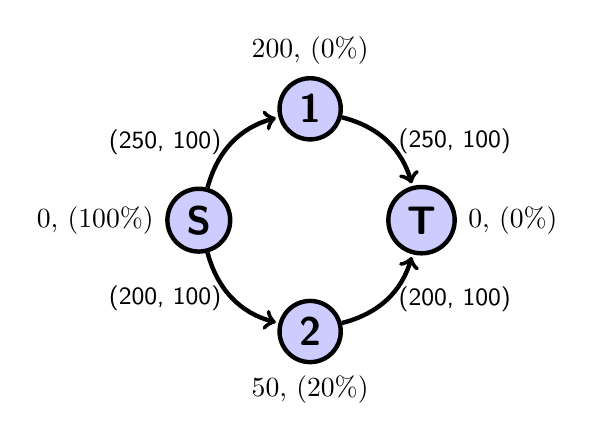
\begin{tikzpicture}[
->,
->,
shorten >=1pt,
auto,
node distance=2cm,
ultra thick,
main node/.style={circle,
								fill=blue!20,
								draw,
								font=\sffamily\Large\bfseries}]
%1
  \node[main node] (1) {1};
  \node[above] at (1.north) {200, (0\%)};
%2 
 \node[main node] (2) [below left of=1] {S};
  \node[left] at (2.west) {0, (100\%)};
%3 
 \node[main node] (3) [below right of=2] {2};
  \node[below] at (3.south) {50, (20\%)};
%4 
 \node[main node] (4) [below right of=1] {T};
  \node[right] at (4.east) {0, (0\%)};
%paths
  \path[every node/.style={font=\sffamily\small}]
    (1)
      edge [bend left] node[right] {(250, 100)} (4)
    (2) edge [bend right] node[left] {(200, 100)} (3)
          edge [bend left] node[left] {(250, 100)} (1)
    (3) edge [bend right] node[right] {(200, 100)} (4)
    (4) ;
\end{tikzpicture}
\label{fig:simpleroad-network}
\caption{A simple road-network with starting point s and end point t. Charge rate dictates that the longer path is the fastest}
\end{figure}

\begin{figure}
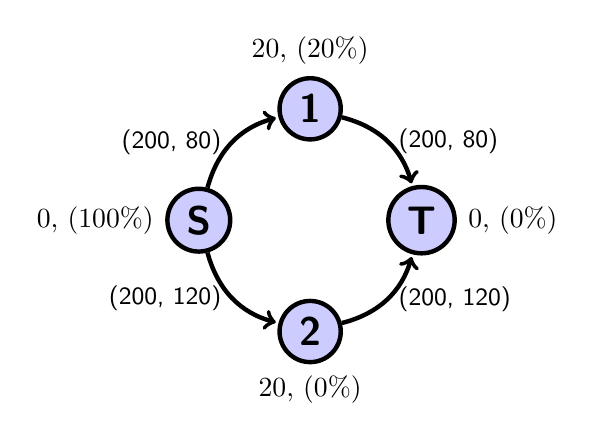
\begin{tikzpicture}[->,->,shorten >=1pt,auto,node distance=2cm,
 ultra thick,main node/.style={circle,fill=blue!20,draw,font=\sffamily\Large\bfseries}]
%1
  \node[main node] (1) {1};
  \node[above] at (1.north) {20, (20\%)};
%2 
 \node[main node] (2) [below left of=1] {S};
  \node[left] at (2.west) {0, (100\%)};
%3 
 \node[main node] (3) [below right of=2] {2};
  \node[below] at (3.south) {20, (0\%)};
%4 
 \node[main node] (4) [below right of=1] {T};
  \node[right] at (4.east) {0, (0\%)};
%paths
  \path[every node/.style={font=\sffamily\small}]
    (1)
      edge [bend left] node[right] {(200, 80)} (4)
    (2) edge [bend right] node[left] {(200, 120)} (3)
          edge [bend left] node[left] {(200, 80)} (1)
    (3) edge [bend right] node[right] {(200, 120)} (4)
    (4) ;
\end{tikzpicture}
\label{fig:simpleroad-network}
\caption{A simple road-network with starting point s and end point t. Consumption rate dictates that the longer path is the fastest}
\end{figure}

A shorter path does not necessarily imply a faster path for electrical vehicles. This is partly due to the fact that electrical vehicles use polynomially more energy as its speed increases but also due to the fact that charge times on charge stations varies a lot. 
Driving a longer path with a fast charge station on, can therefore turn out to be a faster choice than driving a shorter path with a slow charge station on. This is illustrated in Figure \ref{fig:simpleroad-network}. In the example, we assume our car has a battery capacity of 100 kWh and a consumption rate of 0,4 kWh/km at the speed of 100 $\si{\km\per\hour}$. Path 1 consist of two edges with distance: $ 250 \si{\km}$ and speed limit: $100 \si{\km\per\hour}$
and a charge station with a charge speed of 200 kW. Path 2 consist of two edges with
distance: $200 \si{\km}$ and speed limit: $100 \si{\km\hour}$ and a charge station with a charge speed of $30\si{\kW}$. The current battery capacity of the vehicle is noted at each vertex in parenthesis. The total time of each path:
				
\textbf{Path 1:} $\frac{250\si{km} + 250\si{km}}{100\si{\km\per\hour}} + \frac{100\si{\kWh}}{200\si{\kW}} = 5.5\si{\hour}$

\textbf{Path 2:} $\frac{200\si{km} + 200\si{km}}{100 \si{\km\per\hour}} + \frac{60 kWh }{ 30 kW} = 6\si{\hour}$

\todo[inline]{mention other factors which dictates the fastest path}


\section{Related Work}\label{sec:relatedwork}
\todo[inline]{write this}
possible subjects
\begin{itemize}
    \item hierarchies in the graph for faster shortest path
    \item shortest path (dijkstra)
    \item ...
\end{itemize}


\section{Fastest Path}

As we showed in \Cref{sec:shorternotfaster}, finding the fastest path for an EV, from vertex $s$ to $t$ in a road network, does not only depend on the lengths and speed limits of the road network's edges but also on the charge rates of it's vertices. In this section we first describe this path-optimization problem in section \ref{sec:optiprob}. Then we go on to the globally optimal solution in section \ref{sec:LP} and finally we present a greedy heuristic path optimizing algorithm in section \ref{sec:greedy}.

\subsection{Optimisation Problem}\label{sec:optiprob}
This section introduces a formal description of the fastest path problem, modelled as an optimization problem.

\begin{figure}[h!]
\centering
    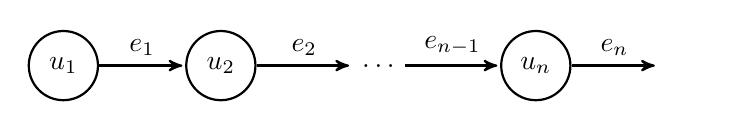
\begin{tikzpicture}[shorten >=1pt,node distance=2cm,>=stealth',thick]
        \node[state] (1) {$u_1$};
        \node[state] (2) [right of=1] {$u_2$};
        \node[] (dots) [right of=2] {$\dots$};
        \node[state] (n) [right of=dots] {$u_n$};
        \node[state,draw=none] (d1) [right of=n] {};
        \draw [->] (1) to[right] node[auto] {$e_1$} (2);
        \draw [->] (2) to[right] node[auto] {$e_2$} (dots);
        \draw [->] (dots) to[right] node[auto] {$e_{n-1}$} (n);
        \draw [->] (n) to[right] node[auto] {$e_n$} (d1);
    \end{tikzpicture}
    \caption{Example of a path consisting of $n$ edges} \label{fig:pathexample}
\end{figure}

The objective of the optimisation problem is to minimise the time spent driving
and the time spent charging on a path from $s$ to $t$. The total time spend driving from $s$ to $t$ can be expressed as follows:
\begin{equation*}
\begin{aligned} &
{\text{min:}}
& & \sum_{i=1}^{n} \left(\frac{D(e_i)}{v_{e_i}} + CT_{u_i} \right)\\
\end{aligned}
\end{equation*}\label{eq:objfunction}
Where $D(e_i)$ is the distance of road segment $i$, $v_{e_i}$ is the speed driven on road segment $i$ and $CT_{u_i}$ is the time spent charging at the $i^{\text{\tiny th}}$ vertex of the path. It should be clear that the objective function of this problem is concerned with time, being that $\frac{D(e_i)}{v_{e_i}}$ is the time spent driving and $CT_{u_i}$ is the time spent charging. The objective function has two unknown variables $v_{e_i}$ and $CT_{u_i}$. The unknown variables of the objective function are constrained by the physical properties of the $EV$ driving the path.

On every edge the speed of the EV must be within the speed limits. $v_{e_i}$ is the speed on edge $e_i$. $v_{min}(e_i)$ and $v_{max}(e_i)$ is the minimum and maximum speed. Thus, the first constraint is formulated as:
\begin{equation*}
\forall_{i\in1 \dots n }:\;v_{min}(e_i) \leq v_{e_i} \leq v_{max}(e_i)
\end{equation*}
The battery level of the EV, must be between $0$ and $B_{max}$, the battery capacity of the vehicle.
This constraint is split in to two constraints. The first constraint ensures that the EV can not pass an edge without having the required energy. The second constraint ensures that the EV can not overcharge at any charging station.
\begin{equation*}
\forall_{i\in1 \dots n }:\; EC(u_i) = R_{CH}(u_i) * CT_{u_i}
\end{equation*}
$EC(u_i)$ is the energy acquired at the $i^{\text{\tiny th}}$ vertex of the path. The energy acquired is calculated as charge speed($R_{CH}(u_i)$) multiplied by charge time($CT_{u_i}$)
\begin{equation*}
\forall_{i\in1 \dots n }:\; ES(e_i) = D(e_i)*R_{CO}(v_{e_i})
\end{equation*}
$ES(e_i)$, the energy spent driving $e_i$, is calculated by multiplying the distance of $e_i$ $(D(e_i))$ by the consumption rate of the vehicle driving at speed $v_{e_i}$ $(R_{CO}(v_{e_i}))$

The EV can not pass an edge without having the required energy. The sum of energy acquired at the charging stations prior to the edge must be larger then the sum of energy used on the edges prior to the edge plus the energy the edge needs. As shown in \Cref{fig:pathexample} vertex $i$ is prior to edge $i$ and the path have the same amount of edges and vertices.
\begin{equation*}
\forall_{i\in1 \dots n }:\;0 \leq B_{cur} + \sum_{j=1}^{i} EC(u_j) - ES(e_j) \leq B_{max}
\end{equation*}\label{eq:energyreq}
$B_{cur}$ is the battery level of the EV at the start of the path, $ \sum_{j=1}^{i} EC(u_j)$ is the amount of energy acquired on the $j^{\text{\tiny th}}$ vertex and all vertices prior to vertex $i$ and $\sum_{j=1}^{i} EC(u_j)$ is energy used on edge $j$ and all edges prior to the $j^{\text{\tiny th}}$ edge.

The EV is not overcharged at any charging station, this constrain looks one charging station further to ensure the energy is balanced before and after passing an edge.
\begin{equation*}
\begin{aligned}
\forall_{i\in1 \dots n-1}:\;0 \leq B_{cur} + \sum_{j=1}^{i+1} EC(u_j) - \sum_{j=1}^{i} ES(e_j) \leq B_{max}
\end{aligned}
\end{equation*}
The values of the constraint is the same as in equation \ref{eq:energyreq}. It should also not be possible for the EV to spend a negative amount of time at a charging station:
\begin{equation*}
\forall_{i\in1 \dots n }:\; 0 \leq CT_{u_i}
\end{equation*}


\subsection{Greedy Heuristics Algorithm}
\todo[inline]{introductory text}

\subsubsection*{Idea outline}
The idea of the approach taken in this section, is using Dijkstra's algorithm for finding the shortest path with $\frac{distance}{speed}$ as the weight of an edge. The problem then becomes, which speed must we use in the interval of $v_{min}$ and $v_{max}$. As argued previously, the optimal speed to drive can only be found by iterating over all possibilities which is a combinatorial optimization problem, and it is NP-Hard. Thus we introduce a heuristic, which promotes local optimal choices. This gives a fast path, but this might not be drivable, if there are not any charge stations on this path, thus we will need to figure out how to incorporate this.\\

We will now analyse how the weight can be found, specifically the speed. The time spent passing an edge $e = (u_1, u_2)$ in the road network, is given by the following equation:
\begin{equation*}
\begin{aligned}
 & T(v,(u_1, u_2)) = \frac{D((u_1, u_2))}{v} + \frac{R_{CO}(v) * D((u_1, u_2)) - B_{cur}}{Best_{CH}(u_1)}
\end{aligned}
\end{equation*}\label{eq:drivingAndCharging}

where $v$ is the speed of the vehicle, $D(u_1, u_2)$ is the distance between vertices $u_1$ and $u_2$, $R_{CO}(v)$ is the consumption rate of the vehicle at the speed $v$, $B_{cur}$ is the current battery capacity of the vehicle and $Best_{CH}(u_1)$ is the charge rate of the best charge station previous to $u_1$ or the charge rate ofs $u_1$.The above equation yields a function on the form: $av^2 + bv + c$, due to the fact that $R_{CO}(v)$ is a quadratic function. $a$ , $b$ and $c$ are some constants which are given by the instance of the vehicle. 
Represented in a Cartesian coordinate system, $T(v,(u_1, u_2)))$ is a parabola, as can be seen in Figure \ref{fig:graph}. On the x-axis is the speed of the vehicle and on the y-axis is the time spent. The turning point of the graph represents the optimal speed to drive at for the given edge, denoted as $v_{opt}(e)$. The point is easily calculated by finding a tangent line with a slope of $0$. If $v_{opt}(e)$ is smaller than $v_{min}(e)$, then $v_{min}(e)$ defines the optimal speed for the edge. Similarly if $v_{opt}(e)$ is larger than $v_{max}(e)$, $v_{max}(e)$ defines the optimal speed for the edge.\\


\begin{figure}[!htb]
\label{fig:graph}
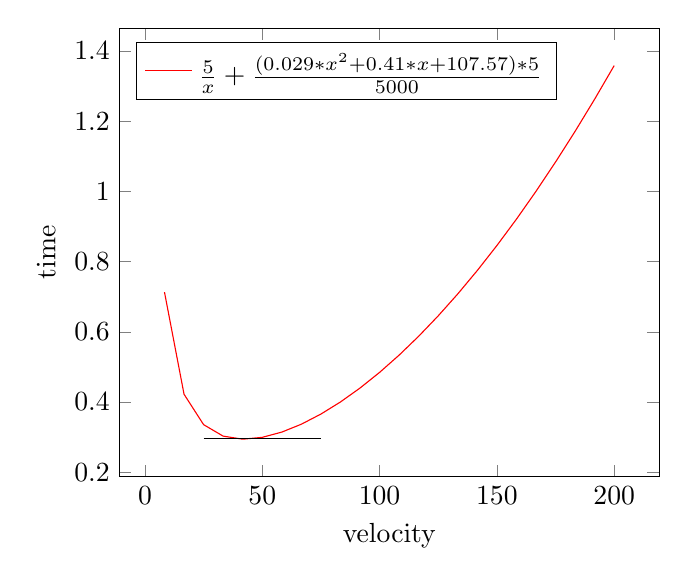
\begin{tikzpicture}
\begin{axis}[xlabel=velocity, ylabel=time,legend style={legend pos=north west}]
\addplot[draw=red,domain=0:200]{(5/x)+(((0.0286*x^2 + 0.4096*x + 107.57)*5)/5000)};
\addlegendentry{$\frac{5}{x}+\frac{(0.029*x^2 + 0.41*x + 107.57)*5}{5000}$}

\addplot[draw=black,domain=25:75]{0.295};
% \addplot[mark=*, domain=25:75] coordinates {(37,295)};
\end{axis}
\end{tikzpicture}% 
\caption{In this instance of $T(v,(u_1, u_2))$, going from $u_1$ to $u_2$, we have a distance of $5 \si{\km}$ and a charge speed of $5 \si{\kW}$ on $u_1$. The optimal speed in this case is $42.12\si{\miles\per\hour}$, which takes roughly 7 minutes to drive}
\end{figure}





While the algorithm progresses through the graph, it need to store a subset of the charge stations on the current path. At every reached charge station, we record the possible energy$B_{possible}$ we can add to the system, defined by $B_{cap}-B_{cur}$ and the charge rate of the station as a tuple: $(B_{possible}, R_{CH}(vertex))$.\\
We maintain a subset of tuples on every vertex by using a list of tuples only with $B_{possible}$ above 0. This will of course always be the case when we reach a charge station, but as we progress through the graph and some distance is being traveled, the possible energy at each previous charge station decreses. The first tuple in the list will always be the the charge station with the best charge rate. A tuple is removed either when $B_{possible}$ hit 0, or when new tuple, with a higher charge rate is found. We make sure to store the best charge station at position 0 in the list, by remove every tuple between the first and second best charge rate in the list.\\

Using this we can define a fastest path algorithm in the following way: \\

\begin{algorithmic}
\Function{GreedyHeuristic}{$RN,s,t,EV$}
	\ForAll{$v \in RN.V$} 
		\State $v.time = \infty$
		\State $v.predecessor = NIL$
		\State $v.preCS = NIL$
		\State $v.B_{cur} = NIL$
	\EndFor
	\State $s.time = 0$
	\State $s.B_{cur} = EV.B_{cur}$

	\State $Q = PriorityQueue$
	\State $INSERT(Q, (s.time, s))$	
	\While{$Q \neq \emptyset$} 
		\State $u = extract-min(Q)$
		\ForAll{each vertex $v \in RN.adj(u)$} 
			\State $time,preCS,B_{cur},energy = travel\_time(RN, u, EV)$
			\If{$v.time > u.time + time$} 
				\State $v.time = u.time + time$
				\State $v.predecessor = u$
				\State $v.B_{cur} = B_{cur}$
				\State $v.preCS = preCS$
				\State $insert(Q, (v.time, v))$	
			\EndIf

		\EndFor
	\EndWhile
	\State \Return $t.time, t.path$
\EndFunction
\end{algorithmic}\label{alg:fastest_path}




\subsection{Approximating an Optimal Path}\label{sec:LP}
In this section an approach to finding a global optimal solution to the optimisation problem proposed in Section \ref{sec:optiprob} is formulated. The optimisation problem is a non-linear optimisation problem, due to \( D(e_i)/v_{e_i} \) and $R_{CO}(v_{e_i})$ being non-linear functions. The problem can however be reformulated as a linear programming problem by formulating \( D(e_i)/v_{e_i} \) and $R_{CO}(v_{e_i})$ as a piecewise-linear functions. Precisely the problem is modelled as a mixed integer problem (MIP) problem. This section introduces the constraints necessary to solve the problem as a MIP problem and thereby end up at an almost global optimal solution. The quality of the solution depends on how many pieces the non-linear function is split into. 

\subsubsection{Linearization}
The linearization of a function is handled as show in \Cref{fig:linearization_example} the none-linear function is split into a number of linear pieces. To handle the linearization three new sets are introduced, a set of known variables which is the pre computed function of each linear piece, and another set of known variables which is the start and end points of each line segment and a set of unknown variables which will be the line segment chosen. The unknown variable is called SL(selected line) and must be a two dimensional of size $n \times m$ where $n$ is the length of the path, each edges has a unique function. $m$ is the number of linear lines the function is split into. This lead to the following constraints.  

\begin{figure}[h!]
\centering
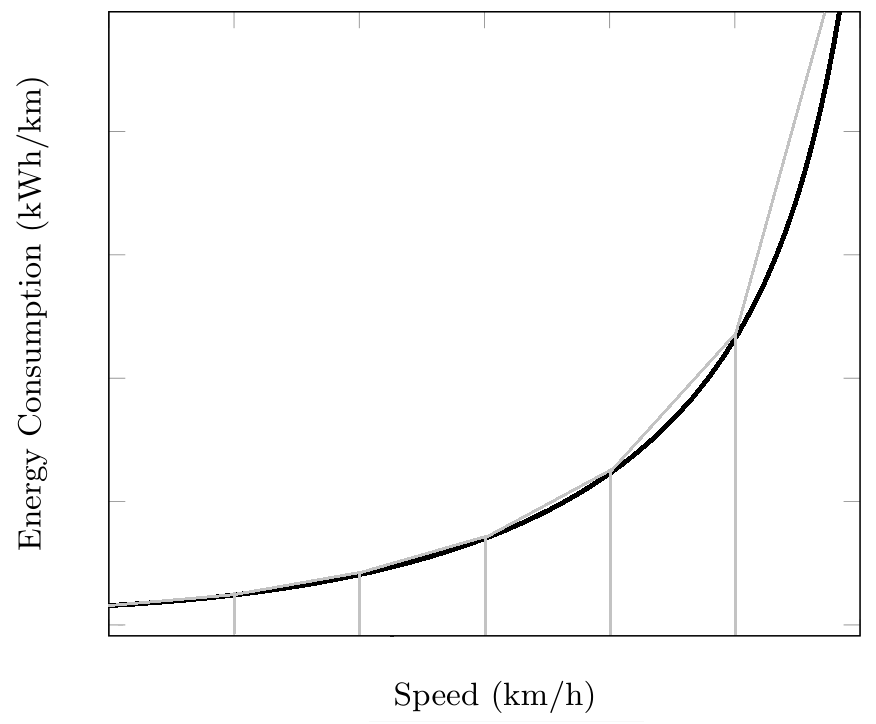
\includegraphics[scale=0.33]{images/linearization_example}
\label{fig:linearization_example}
\caption{Example of a non-linear function which is split into 6 pieces}
\end{figure}

Exactly one line segment needs to be selected for all line segments. 
\begin{equation*}
\forall_{i\in1 \dots n }:\; \sum_{j=1}^{m} SL_{i,j} = 1
\end{equation*}

$n$ is the length of the path, $m$ is the amount of lines the functions \( D(e_i)/v_{e_i} \) and $R_{CO}(v_{e_i})$ are split into and $\sum_{j=1}^{m} SL_{i,j} = 1$ ensures that only one line segments can be selected.
Being that exactly one line segment needs to be chosen. In other words, SL needs to be binary values.
\begin{equation*}
\forall_{i\in1 \dots n, j \in 1 \dots m}: \; \; SL_{i,j} \in{0,1} 
\end{equation*}
The speed of the EV needs to be constrained by the line segment chosen:
\begin{equation*}
\forall_{i\in1 \dots n, j \in 1 \dots m-1}:\; SL_{i,j} * P_{i,j}  \le  v_{j,e_i} \le SL_{i,j}*P_{i,j+1}
\end{equation*}

$P$ is a set of starting points of all line segments including the end point of the last segment. $SL_{i,j} * P_{i,j}$ is the minimal speed the EV is allowed to drive on edge $i$ and $SL_{i,j}*P_{i,j+1}$ is the maximal speed, note that the values will either be a valid value or $0$ if the segment is not selected. $P_{i,j+1}$ is the end point of $P_{i,j}$. 
The approximate solution to \( D(e_i)/v_{e_i} \) or $R_{CO}(v_{e_i})$ can now be found by precomputing the functions of each of the individual linear lines \( D(e_i)/v_{e_i} \) or $R_{CO}(v_{e_i})$ is split into, the produce precomputing is a set of slopes called $LinesA$ and a set constants called  the  multiplying the slope of the selected line with the selected speed and adding the constants called $LinesB$. As an example the way to model $R_{CO}(v_{e_i})$ for $i$
\begin{equation*}
\sum_{j=1}^{m} LinesA_{i,j}*v_{j,e_i} + \sum_{j=1}^{m} SL_{i,j}*LinesB_{i,j} 
\end{equation*}
$\sum_{j=1}^{m} LinesA_{i,j}*v_{j,e_i}$ is equlent of $a*x$ and $\sum_{j=1}^{m} SL_{i,j}*LinesB_{i,j}$ is equivalent with $b$ and thus the consumption rate of the EV is modeled as $m$ function in linear form $a*x + b$. 
Finally note that this is a way to determine the solution of \( D(e_i)/v_{e_i} \) or $R_{CO}(v_{e_i})$ and before the solution can be found the line segments and points for each of both of the non linear functions needs to be precomputed. 
%sources
%1, SWP-3587
%2, glpk-sos2




\section{Experiments}
\label{sec:experiments}
Now we present the experiments of the Greedy Heuristic Algorithm. It was concluded that the practical usage of the linear programming solution was not plausible in our experiments, after several implementations using an existing solver. Additionally, there will be a runtime complexity test of the algorithms.

We have constructed four experiments, to figure out what implication the adjusting of these parameters will have on the Greedy Heuristic Algorithm. The four parameters being experimented on are:
\begin{itemize}
     \item Route driving distance
     \item Charge rate of charge stations
     \item Consumption rate of EVs
     \item Density of charge stations
 \end{itemize} 

\todo[inline]{insert default values}


\subsection{Road network dataset} 
\label{sub:setup}
To facilitate the experiments, we've had to find a real world road network dataset which contains road distances, speed limits and charge stations of varying charge rates. Such a dataset does not openly exist to our knowledge. Instead we have used OpenStreetMaps which is an open-source collection of map data. One can read more about OSM at \url{http://www.openstreetmap.org/about}. OSM has a concept of ways and vertices. Ways represent geographical planar objects e.g. roads, cycleways, foot ways etc. A vertex is a geographical point consisting of a latitude and longitude coordinate. A way is constituted of a set of vertices and some tags which describe meta-information about the way, such as the name of the way and what type of way it is e.g. a road, cycleway, foot way  etc. From this information we can derive that if way $e_1$ and $e_2$ intersect in vertex $u$, they will share the vertex $u$. A vertex is referred to as either a road intersection or as a charge station if the vertex has been assigned a charge rate.\\

The ways and vertices can easily be converted into a, for us, useful road network structure for experimenting. This is done, by simply filtering away all types of ways accept roads and use these as edges in the road network. To get a notion of speed limits on edges, we derive general speed limits from the type of the roads. OSM carries such information as whether the road is a motorway, residential way, tertiary way etc. The speed limits are set according to Danish speed limits. For vertices, we are only interested in the ones which correspond to intersections between two roads. All other vertices in the road network are ignored. To get a notion of charge rate on the vertices we have implemented a method which distributes random charge rates on randomly selected vertices in the road network.\\

We have used the drivable part of Denmark as a baseline for the experiments. The dataset features:
\begin{itemize}
    \item 483407 vertices
    \item 543482 edges
\end{itemize}

\subsection{Naive algorithm}
\label{sub:naivealgorithm}
We have formulated a naive algorithm for performance comparison with our greedy-heuristic algorithm. The naive algorithm should simulate the way a naive electric vehicle driver would choose to travel through a road network. The naive algorithm works the following way: It greedily chooses the fastest roads in terms of distance over speed. Whenever the battery reaches 40 \% battery capacity, it starts searching for nearby charge stations in the radius allowed by the 40 \% battery capacity given the vehicles consumption rate. If no charge stations are available with 40 \% battery capacity, the path from $s$ to $t$ is not solvable for the naive algorithm. If, on the other hand, one or more charge stations are reachable, the algorithm will choose the closest one and charge to 100 \% battery capacity or to the battery capacity needed in order to reach $t$. After charging, the algorithm will resume greedily choosing the fastest roads from the charge station to $t$, in terms of distance over speed.

\subsection{Experiment: Complexity of Road Network}

We compared the run-time of the Greedy-heuristic algorithm to the naive algorithm with the complexity of the road network as changing parameter. The
complexity is measured in the number of vertices on the road network. The more vertices on the road network, the more vertices the two algorithms has 
to visit before they are able to find a fastest path. The set-up of the experiment: distance to drive was 100 km, the minimum distance between 
charge stations was 20 km. The initial number of vertices in the road network: 450000 vertices. The number of vertices is then counted down with 10000 for each iteration of the test. The resulting graph is illustrated in (REF!).

\subsection{Experiment: Density of Charge Stations}

We compared the performance of the Greedy-heuristic algorithm to the naive algorithm with the density of charge stations as changing parameter. The
density of charge stations are measured in the minimum distance between two charge stations. Initially, the minimum distance is set to 5 km which generates 3029 charge stations in Denmark. Table \ref{table:chargedensity} shows the number of charge stations according to the minimum distance between charge stations in the road network.

\begin{table}[!htb]
\centering
		\begin{tabular}{ p{1.85cm} p{0.67cm} p{0.63cm} p{0.63cm} p{0.63cm} p{0.63cm} p{0.63cm} } \hline
		Radius (km): & 5 & 10 & 20 & 30 & 40 & 50 \\ \hline
		Stations: & 3029 & 827 & 326 & 117 & 76 & 49 \\ \hline 
		\end{tabular}
		\caption{number of charge stations corresponding to the minimum distance between two charge stations}
	\label{table:chargedensity}
	\end{table}

The set-up of the experiment: the distance to drive was set to 200 km, the complexity of the road network was 483398 vertices, which is the number of vertices in Denmark. The charge rates of the charge stations are evenly distributed with rates between $10 \si{\kW}$ and $100 \si{\kW}$. The resulting graph is illustrated in (REF!).

\subsection{Experiment: Charge Rate on Charge Stations}

We compared the performance of the Greedy-heuristic algorithm to the naive algorithm with the charge rate of charge stations as changing parameter. The minimum distance between charge stations was set to 30 km, the distance to drive was set to 200 km. The initial charge rates in the road network were evenly distributed between $10 \si{\kW}$ and $100 \si{\kW}$. For each iteration all charge rates are scaled with a constant factor resulting in worse of better charge rates on all charge stations. The resulting graph of the experiment is seen in (REF!). On the x-axis is displayed the average charge rate of the charge stations on the road network. On the y-axis is displayed the time it takes to pass a path of length 200 km. 

\subsection{Experiment: Size of Road Network}



\subsection{Citations}

\section{Conclusion}
\label{sec:conclusion}
As the adoption rate of EVs increases time-optimised route planning systems for electrical vehicles will become increasingly important. 
We showed that a route planning system for EVs should take charging stations and charging rates into account, since the time spend 
charging an EV with today's standards is still relatively long. 

The problem of finding a route plan for an EV can be modelled as an optimisation problem. We implemented a greedy heuristic algorithm that used greedy choices and heuristics about the EV and the road network to find time-optimised paths. We ran several experiments on a real world road network and compared the performance with a naive algorithm that simulated the pattern of a naive electric vehicle driver. The experiments showed that the greedy heuristic algorithm both finds better paths and better charging plans than the naive algorithm. The worst-case time complexity of the greedy heuristic algorithm is $O(|V||E|+|V^2|\log|V|)$

We further implemented a linear programming solution using GNU Linear Programming Kit but found that solving every simple path in a graph with the size of a real world road network, is simply too expensive to compute within reasonable time. We compared the path time outputted by the greedy heuristic algorithm to the path time of the linear programming solution when run on the same path. \todo[inline]{How good are the paths found relative to the linear programming solution?}
  

%ACKNOWLEDGMENTS are optional
%%ACKNOWLEDGMENTS are optional
\section{Acknowledgements}
This section is optional; it is a location for you
to acknowledge grants, funding, editing assistance and
what have you.  In the present case, for example, the
authors would like to thank Gerald Murray of ACM for
his help in codifying this \textit{Author's Guide}
and the \textbf{.cls} and \textbf{.tex} files that it describes.	

\subsection{References}
Generated by bibtex from your ~.bib file.  Run latex,
then bibtex, then latex twice (to resolve references)
to create the ~.bbl file.  Insert that ~.bbl file into
the .tex source file and comment out
the command \texttt{{\char'134}thebibliography}.
% This next section command marks the start of
% Appendix B, and does not continue the present hierarchy

\end{document}
